\documentclass{article}
\usepackage[backend=biber]{biblatex}
\usepackage{graphicx}
\usepackage[colorlinks=true]{hyperref}
\usepackage{booktabs}
\usepackage{siunitx}
\usepackage[]{amsmath}
\usepackage{gensymb}
\usepackage{mathtools}
\usepackage{fancyref}
\addbibresource{/home/giorgio/Bibliography/bibliography.bib}
\hypersetup{
    colorlinks=true,
    linkcolor=blue,
    filecolor=magenta,  
    citecolor=blue,    
    urlcolor=cyan,
    pdftitle={Turbina ad alta temperatura},
    bookmarks=true,
}

\author{Anthony Steven Luna Gonzales, \\Roberto Giusto, Giulia Barbero, Giorgio De Trane}
\title{\textbf{Turbina ad alta temperatura}}

\begin{document}
    \setlength{\parindent}{0pt}
    \maketitle
    \begin{center}
        
\includegraphics[width=0.9\textwidth]{Sources/polito_logo.png}\linebreak\newline
       \textbf{\textit{Materiali per applicazioni aerospaziali}}\linebreak\newline
        \textit{Gruppo di lavoro n. 10B}\linebreak\newline
        \textit{Anno accademico 2020/2021}
    \end{center}

    \newpage
    \tableofcontents
    \newpage
    \section{Introduzione\label{Intro}}
    I turbomotori assiali aeronautici possono essere suddivisi, generalmente, in tre macrosezioni
    fondamentali: compressore, camera di combustione e turbina.\\

    \begin{figure}[h!]
        \centering
        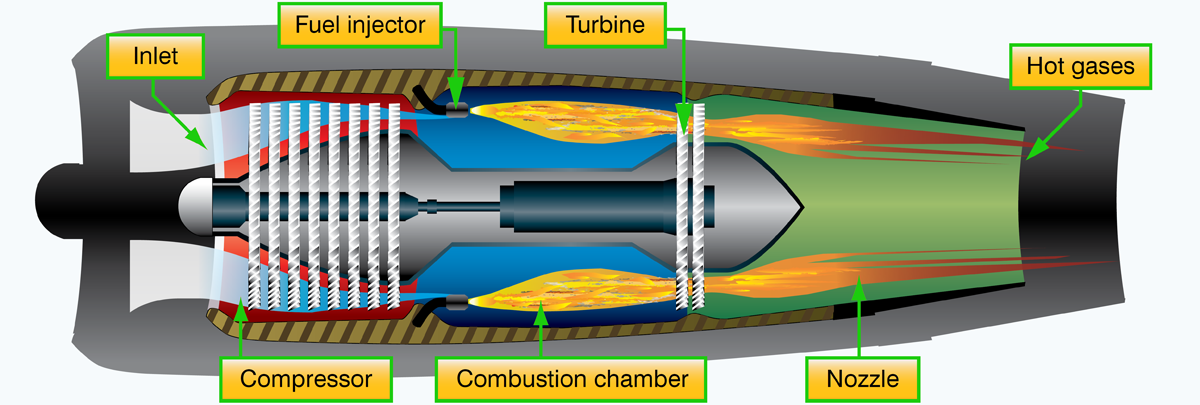
\includegraphics[width=0.8\textwidth]{Sources/turbojet.png}\\
    \caption{Schema generale di un motore turbojet \autocite*{turbojet}} 
    \end{figure}

    Un \textit{inlet} favorisce l'afflusso di aria esterna al \textit{compressore}, il quale
    la comprime in un volume nettamente inferiore, attraverso vari stadi alternati di pale rotoriche-statoriche.\\
    L'aria fortemente compressa viene poi miscelata con il carburante iniettato in \textit{camera di combustione},
    in una determinata proporzione (dipendente da vari fattori): la miscela viene quindi combusta, seguendo le trasformazioni di
    un preciso ciclo termodinamico (ogni motore ha la sua implementazione, ma i principi fondamentali sono gli stessi), causando un repentino
    aumento di pressione e temperatura.\\
    Successivamente, i gas combusti vengono espansi rapidamente dalla \textit{turbina} (la quale, inoltre, mette in rotazione l'albero di trasmissione), attraverso, in questo caso,
    vari stadi alternati di pale statoriche-rotoriche.\\
    Infine, i gas espansi vengono espulsi e accelerati attraverso un \textit{ugello}.\\
    Tutto il processo fornisce una spinta, secondo il principio di azione-reazione \autocite*{Aircr_engine_design}.\\ \\
    Le temperature e le sollecitazioni raggiunte dalle palette di turbina sono tipicamente in range estremi (in particolare per gli stadi ad alta pressione),
    al punto che la scelta dei materiali é sostanzialmente diversa da quella del compressore.\\
    In un moderno jet engine, si possono raggiungere temperature massime che eccedono i 1500 °C \autocite*{SciencePubGroup}, 
    senza contare le sollecitazioni meccaniche a cui sono sottoposte le pale HP, a causa di pressioni elevatissime,
    forze centrifughe per velocitá di migliaia di RPM e intense vibrazioni, nonché problemi di corrosione
    e reazioni chimiche indesiderate, favorite oltretutto dall'alta temperatura.\\

    \begin{figure}
        \centering
        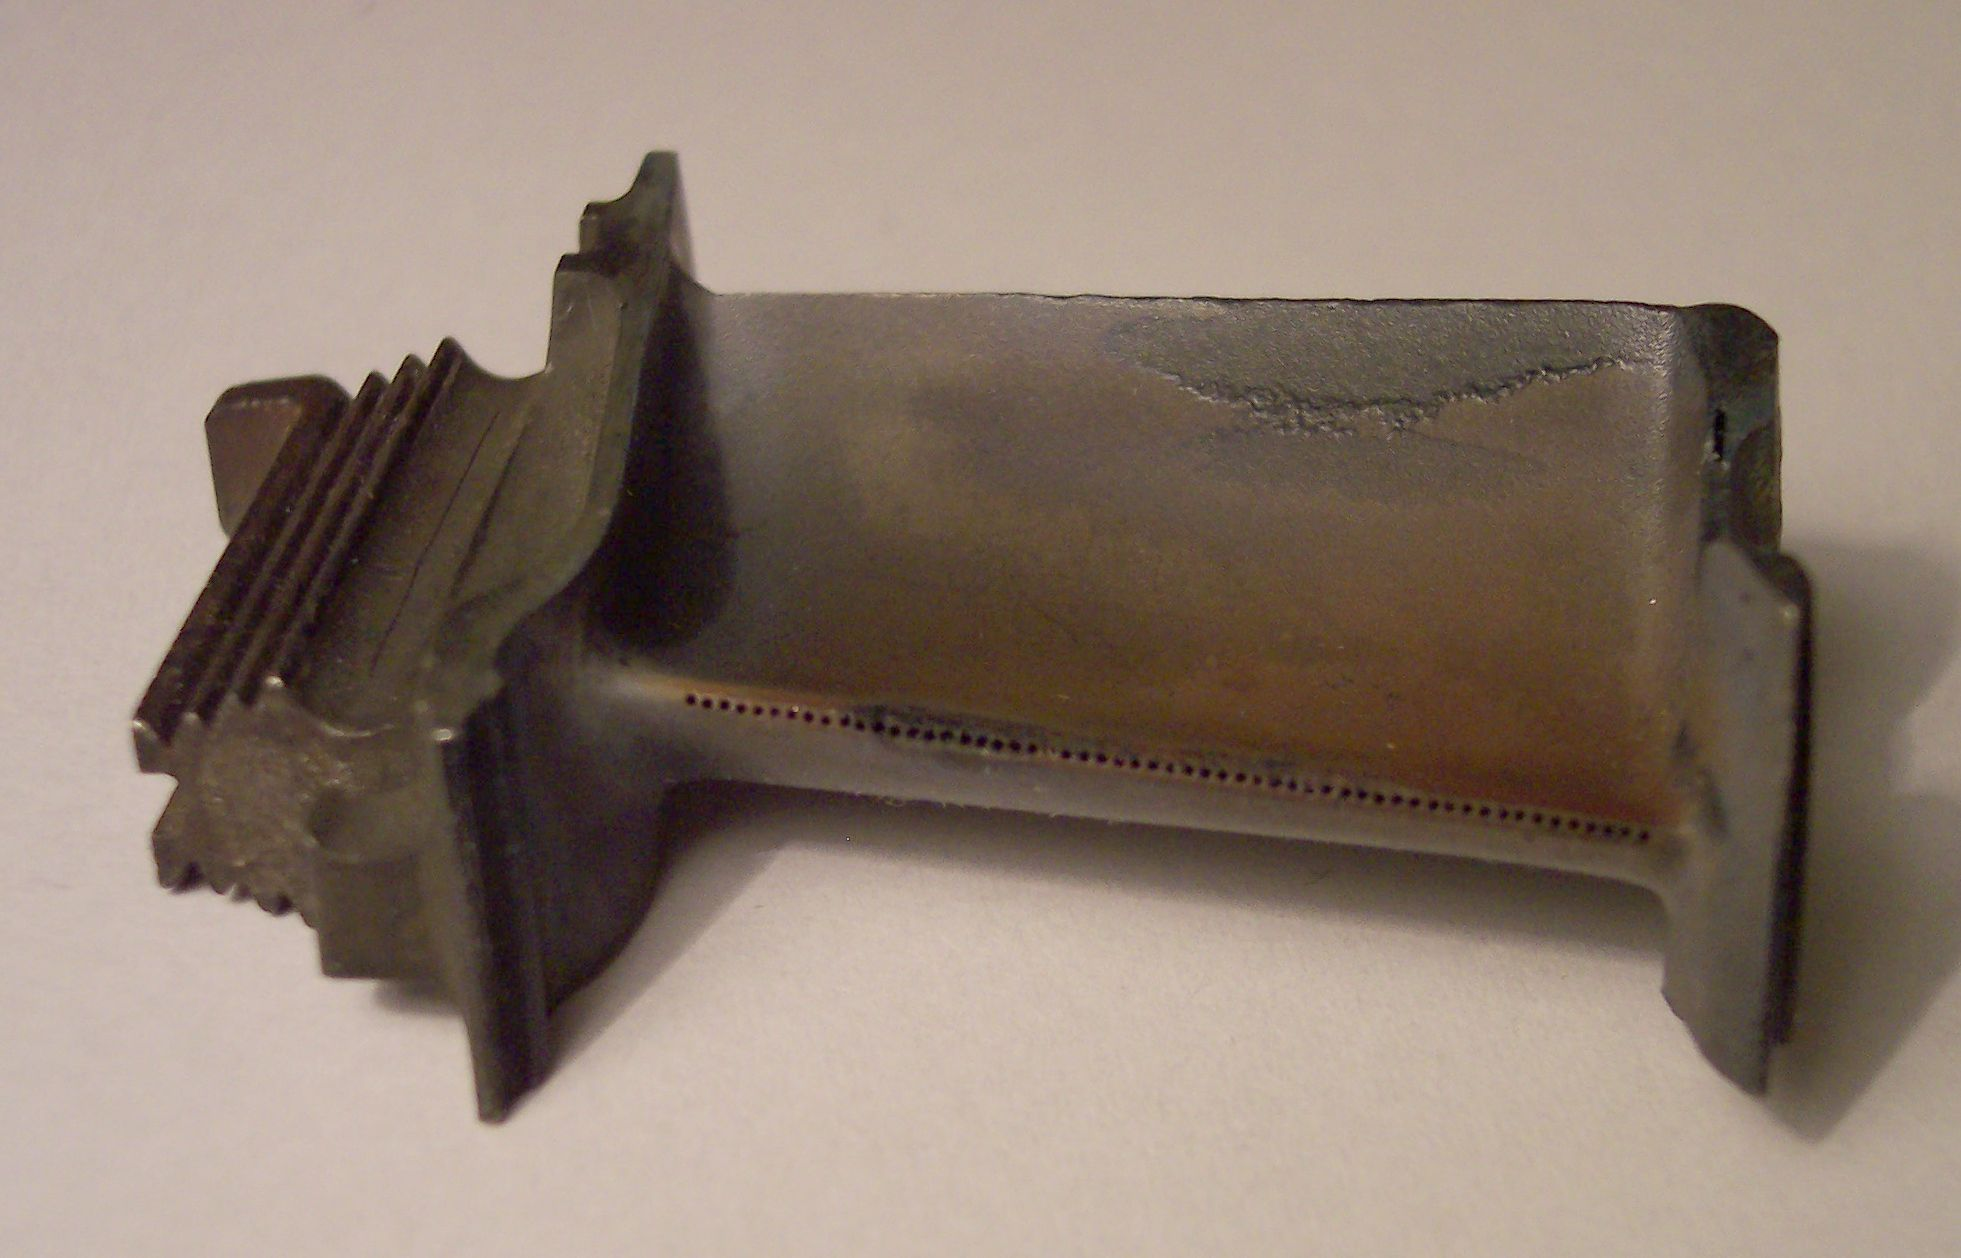
\includegraphics[width=\textwidth]{Sources/Turbinenschaufel_RB199.jpg}
        \caption{Effetti dell'ambiente operativo estremo su una paletta di turbina \autocite*{turbine_blade}}
        \phantomsection \label{fig:paletta_logorata}
    \end{figure}

    É necessario, dunque, scegliere un materiale (o una combinazione di piú materiali)
    in grado di sopportare, per il tempo di operativitá del componente, l'effetto
    simultaneo dell'elevatissima temperatura, dell'aggressivitá chimica e delle sollecitazioni meccaniche istantanee e cicliche,
    tenendo in considerazione, eventualmente, la possibilitá di un raffreddamento attivo.\\

    \pagebreak




    \section{Funzioni, obiettivi, vincoli\label{funz_vinc_ob}}
        \begin{tabular}{l|r}
            \toprule
                \textbf{\textit{Funzione}}   & x\\
                \textbf{\textit{Obiettivi}}  & y\\ 
                \textbf{\textit{Vincoli}}    & z\\ 
            \bottomrule
        \end{tabular}   
        \pagebreak


    \pagebreak


    \pagebreak

    \section{Selezione dei materiali\label{material_selection}}
        \subsection{Stage 1\label{Stage_1}}
        \clearpage
        \subsection{Stage 2\label{Stage_2}}
        \clearpage
        \subsection{Indici di merito\label{material_index}}

        Una buona strategia di analisi qualitativa per la selezione di materiali é rappresentata dalla valutazione di alcuni parametri frazionari, riferiti a una moltitudine di proprietá fisiche, chimiche, termiche, meccaniche, ecc, noti come indici di merito.
        
        Tali indici, definiti ad hoc in base alle necessitá del progettista, consentono di effettuare rapidamente un’indagine comparativa tra una lista di potenziali candidati che hanno superato una fase di preselezione, nel caso in cui la scelta del materiale non sia particolarmente ovvia o scontata. 
        \\ \\
        Nel caso specifico della paletta di uno stadio di turbina ad alta pressione, come giá visto in precedenza, sorgono diverse sfide con requisiti estremi da soddisfare simultaneamente.

        Possono quindi tornare molto utili alcuni indici di merito, dato che devono essere garantiti una elevata temperatura di esercizio, un basso coefficiente di espansione termica, un’alta fracture toughness, un’alta resistenza a fatica, un elevato modulo elastico, un’alta frequenza naturale di risonanza, oltre che un’ottima resistenza all’aggressivitá chimica dell’ambiente operativo. 
        
        Tutti i possibili indici di merito di un materiale sono spesso definiti in funzione della densitá, specialmente in campo aerospaziale, in cui l’ottimizzazione del peso di ogni componente risulta fondamentale, tra le svariate motivazioni, per massimizzare l’efficienza propulsiva, riducendo quindi la spesa sul carburante, che ha un impatto sostanziale sui costi complessivi di un velivolo.
        \\ \\ 
        In seguito alla promettente fase di preselezione sul database,
        superata da sei materiali candidati, si é deciso di concentrarsi su gli indici relativi alla \textit{fracture toughness} e alla \textit{resist fatigue},
        per le quali i materiali preselezionati non mostrano evidenti compromessi ottimali.

        \begin{figure}[h!]
            \centering
            \phantomsection \label{blade_load}
            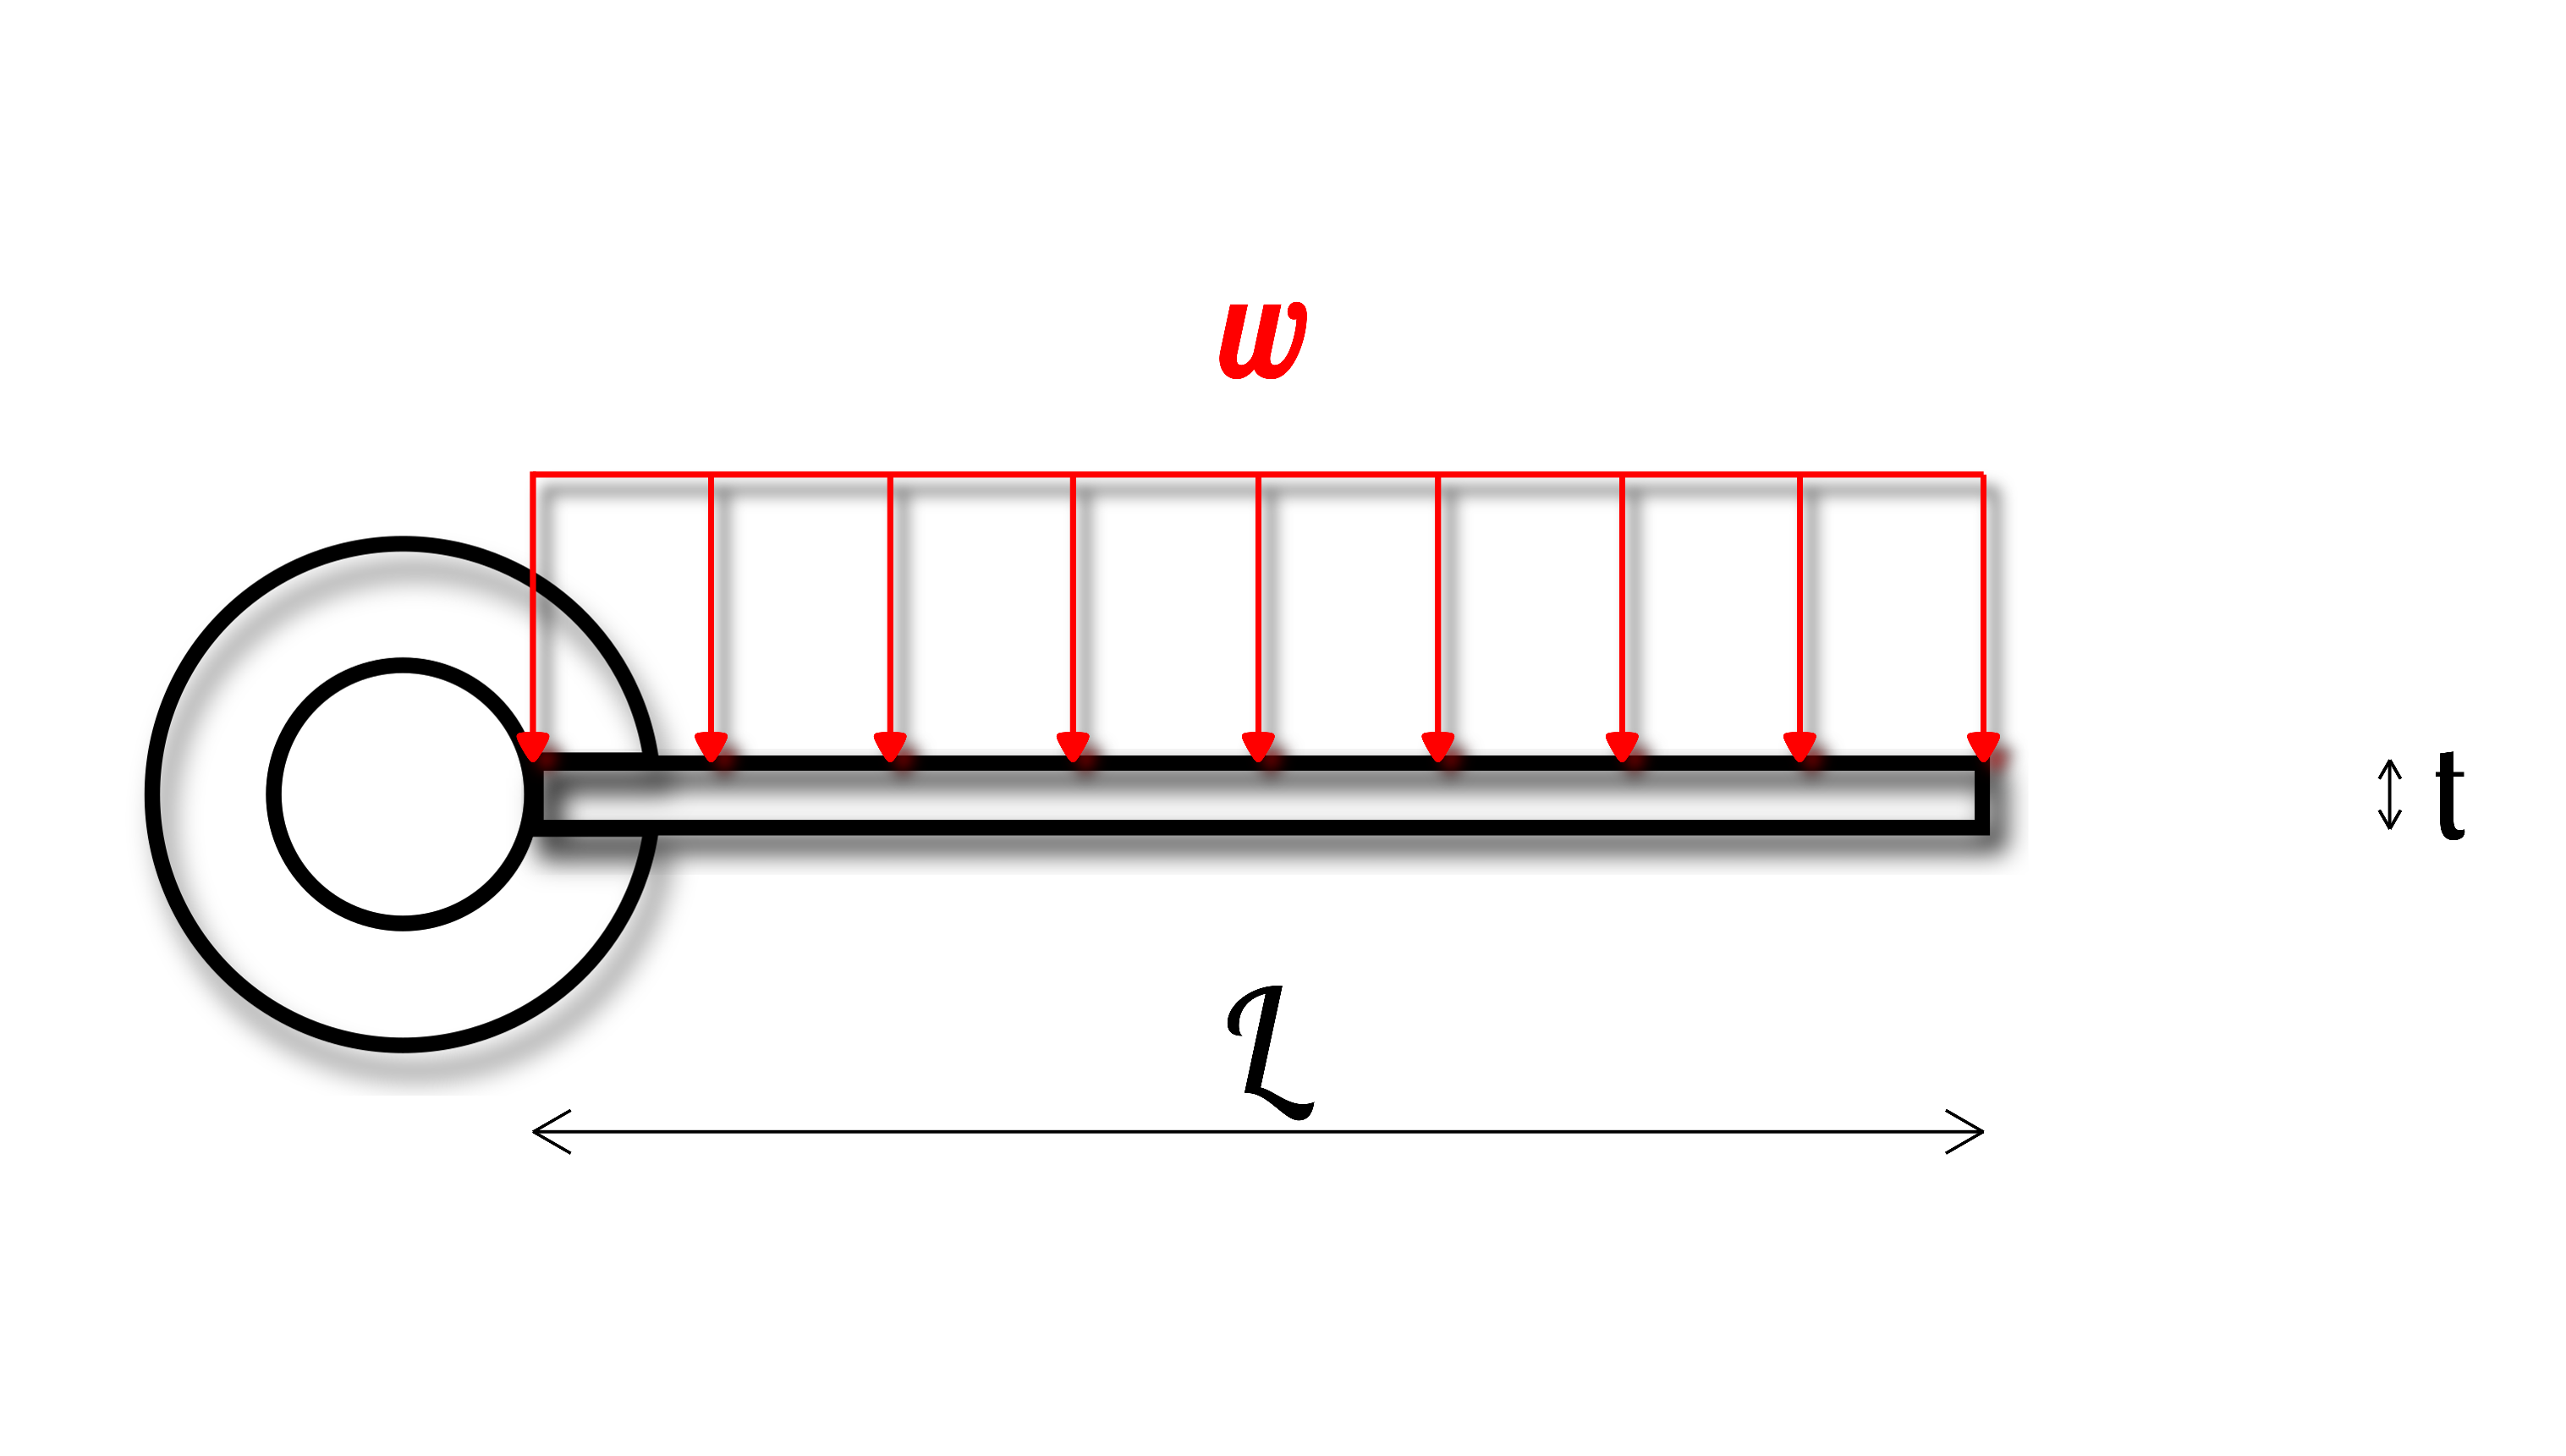
\includegraphics[width=0.8\textwidth]{Sources/blade_load.eps}
            \caption{Schematizzazione semplificata di una paletta \autocite{Inkscape}}
        \end{figure}
        \clearpage

        Per semplificare i calcoli, si assume una paletta rappresentata da una trave a base rettangolare
        estrusa, caratterizzata da:

        \begin{itemize}
            \item Lunghezza \textit{L} [m]
            \item Spessore \textit{t} [m]
            \item Larghezza $\lambda t \ [m]$ (con aspect ratio $\lambda$)
            \item Carico uniformemente distribuito $w = \frac{F}{L}$ [N/m]
            \item Stress applicato $\sigma(y) = \frac{M}{I} \cdot y \ \ \ [\frac{N}{m^2}]$ (dall'equazione di \textit{Navier})
                \begin{itemize}
                    \item $I = \frac{\alpha t^4}{12} \ \ [m^4]$ 
                    \item $M = \frac{wl^2}{2} \ \ [N \cdot m]$
                \end{itemize}
            \item Stress massimo per $\sigma_{max} = \sigma(y = \frac{t}{2})$
            \item Area della sezione $A = \lambda t^2 \ [m^2]$
            \item Densitá $\rho \ [\frac{kg}{m^3}]$
            \item Massa $m = \rho \cdot AL \ \ [kg]$
        \end{itemize}

        Attraverso una manipolazione delle giuste grandezze, gli indici di merito di interesse possono essere ricavati 
        in maniera del tutto indipendente dalla geometria della paletta, focalizzandosi quindi
        sulle proprietá intrinseche del materiale.
        \\ \\ 
        Ipotizzando che la paletta abbia una cricca centrale di dimensioni trascurabili
        rispetto alla sua larghezza, si definisce la \textit{fracture toughness}:

        \begin{equation}
            K_{1c} = \sigma\left(\pi c\right)^{0.5} 
            \phantomsection \label{equation:frac_tough}
        \end{equation}
        dove $\sigma$ é lo sforzo applicato, c é la dimensione della cricca. \\ \\ 

        Manipolando l'equazione con le caratteristiche della paletta precedentemente
        elencate, si ottiene una massa $m \propto \left(\frac{\rho}{K_{1c}}\right) $.

        Alla luce di quanto detto, si definisce il relativo indice di merito, da massimizzare:

        \begin{equation}
            i_{K} = \left (\frac{K_{1c}}{\rho}\right)
            \phantomsection \label{equation:index_frac_tough}
        \end{equation}
        \clearpage 

        Si procede in maniera del tutto analoga per definire un indice di merito relativo alla 
        \textit{resist fatigue}.

        Si definisce una \textit{resist fatigue} (che deve essere il piú alta possibile,
        visto l'onere delle sollecitazioni cicliche a cui é tipicamente sottoposta una paletta di turbina), 
        attraverso la disuguaglianza:

        \begin{equation}
            \sigma_e \geq \frac{wL}{A}
            \phantomsection \label{equation:resist_fatigue}
        \end{equation}

        Dopo varie sostituzioni algebriche, si ottiene una massa $m \propto \frac{\rho}{\sigma_e}$.

        Per cui in definitiva, si definisce il relativo indice di merito, da massimizzare:

        \begin{equation}
            \phantomsection \label{equation:resist_fatigue_index}
            i_{sigma} = \left (\frac{\sigma_e}{\rho}\right)
        \end{equation}

        \clearpage 
        \dots
        \subsection{Stadio N}
        \pagebreak

    \section{Processo Produttivo\label{product_process}}

    \pagebreak

    \section{Conclusioni\label{conclusioni}}

    \pagebreak

    \printbibliography
    
\end{document}
